\section{模型的建立与求解}

\subsection{相似性度量模型}

\begin{figure}[htbp]
    \centering
    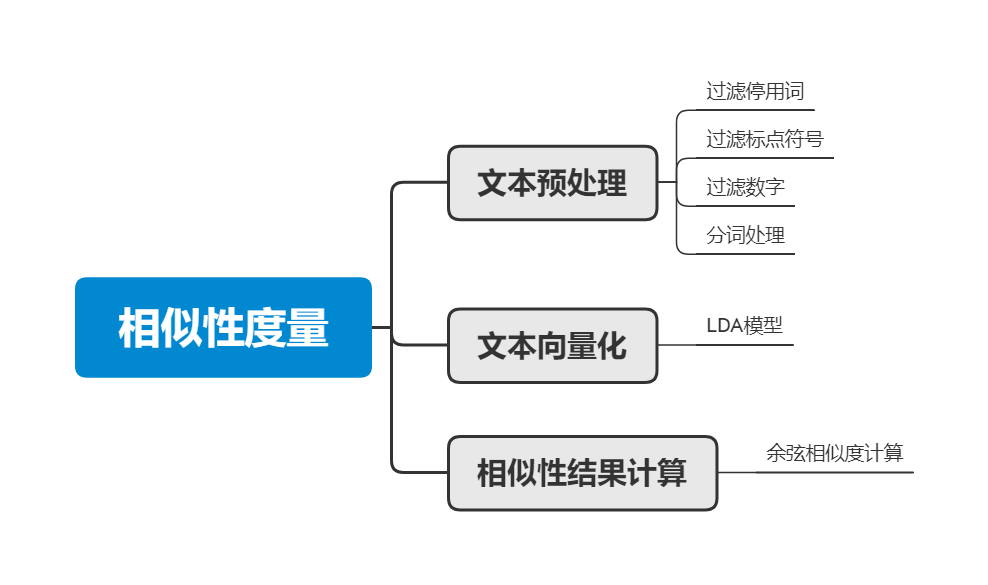
\includegraphics[scale=0.2]{res/figure040956.png}
    \caption{相似度量模型思维导图}
\end{figure}

\subsubsection{度量角度的确立}

在对小学数学应用题的相似性度量过程中,通常会使用两个依据:

\begin{enumerate}
    \item 根据题干文字进行相似性比对,确定两道题目间题面的相似程度。
    \item 通过人工或机器学习的方式为题目根据知识点进行“标签化”,两道题目之间的标签重合越多,则越相似。
\end{enumerate}

实际上,进行“标签化”对题目进行相似性度量是较为科学且准确的,符合师生快速锁定同类题型进行巩固训练的实际需求,而光凭文本信息进行相似性度量的结果并不符合实际的教育需求。

但仅根据少量题目样本无法将“标签化”过程有效自动化,难以避免通过人工手段为题目加上知识点标签。考虑到平台运营的切实情况,人工进行“标签化”操作成本过大,且判断过程中人为主观因素较多,可能也会导致度量结果出现较大偏差。

因而,本文经过综合考虑,还是选择通过题干文字进行相似性比对进行相似性度量。

\subsubsection{度量过程的关键步骤}


本文将度量过程总结成四个关键步骤以便于读者理解,下文也将围绕这四个关键步骤进行展开:

\begin{enumerate}
    \item 文本预处理
    
    文本预处理是自然语言处理中的重要步骤之一,其目的是将原始的文本数据转换成计算机可以处理的形式。为了提高文本处理任务的效率和准确性,文本预处理是在进行后续分析处理的必要前置步骤。

    \item 借助LDA模型向量化题目文本
    
    为了满足平台后续的题库计算需要,必须通过计算机对题目进行大量相似性比对处理。而计算机只能处理数字,文本却是一种非结构化数据,并不能被计算机高效识别处理。因此需要对文本信息进行转换。将文本转换为向量是一种常用的方式,可以将文本表示为数值形式的向量,从而利用向量之间的数学运算来计算文本之间的相似度。

    \item 使用余弦相似度计算相似性结果
    
    经过上述两步的处理后,题目的文字信息已经完成“数学化”,接下来仅需通过数学方法——余弦相似度来对题目间的相似性进行度量。整个题目相似性的度量模型也在此步建立完成。
\end{enumerate}

\subsubsection{文本预处理}

\begin{figure}[htbp]
    \centering
    \label{photo041944}
    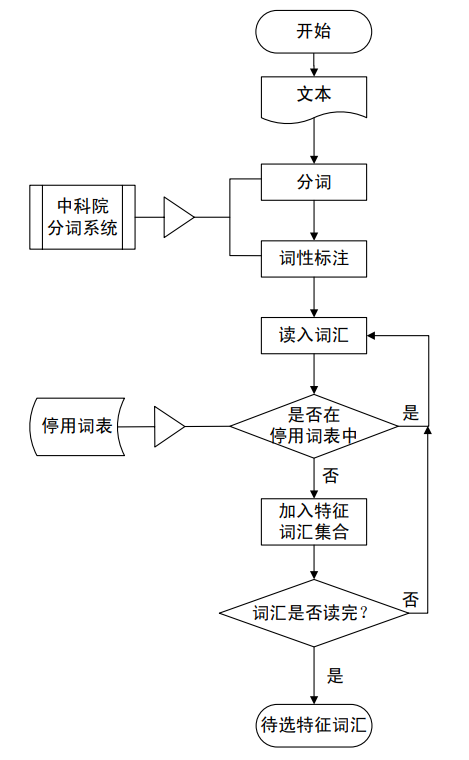
\includegraphics[width=6cm,height=10cm]{res/Text preprocessing process.png}
    \caption{文本预处理流程图}
\end{figure} 

首先需要对题目文本进行分词处理,以好通过词袋模型的方式将题目文本进行向量化,进行进一步的研究。因本文研究的题目大多处于中文语言环境下,需先对题目进行分词处理。本文为了研究方便,使用的是被广泛使用的开源中文分词工具jieba。另外也可以使用NLPIR分词系统达到相同效果。NLPIR分词系统是由中国科学技术大学自然语言处理与社会人文计算实验室开发的一款中文自然语言处理工具。它是基于统计和规则两种方法相结合的分词系统,能够对中文文本进行精准的分词和词性标注,完美契合本文的研究需要。

在分词处理的过程中,还需要分离并忽略标点符号、数字、停用词等词语的影响。详细的处理操作可以参考周萍老师在《语义分析及相似性度量方法》\cite{ZhouJiYuYuYiFenXiDeWenBenXiangSiXingDuLiangYanJiuJiYingYong2017}研究中总结的预处理流程,如\ref{photo041944}。但本文简化了处理流程,仅对分词结果进行了简单的标点符号排除与数字排除,以加快研究进程。

在这里也给出一段进行文字预处理的Python代码以作参考:

\begin{mgCodeBlock}[Python 文字预处理代码]
    \VerbatimInput{res/participle.py}
\end{mgCodeBlock}

\subsubsection{借助LDA模型向量化题目文本}

若仅通过传统方式进行普通的“文字对比”,可以采取TF-IDF分析文本中的关键词再进行相似性度量。但TF-IDF是通过计算文本中每个词的出现频率和在文档集中的逆文档频率来对文本进行编码的一种手段,在过程中没有“主题”这一概念的考量。如果对长篇文章、论文进行检索,TF-IDF算法可以起到很好的度量效果,但针对文本信息较小的小学数学应用题来说,TF-IDF算法并不能良好的将题目进行归类,分析结果可能因题目背景的改变受到严重限制。

因此,本文选用更适合“题目”这一研究对象的度量模型——LDA模型,进行相似性度量。LDA模型可以将题目集合分解为一组潜在的话题,并确定每个题目的话题分布。这些话题可以被视为题目的主题,因此LDA可以用于识别和分析题目集合中的主题和关键词,并确定题目之间的相似性。

相似的,在“在线编程题目推荐算法”的相关研究中\cite{LuoRongHeZhiShiDianYuTuJuanJiDeZaiXianBianChengTiMuTuiJianSuanFa},也选用了LDA模型作为题目相似性的判断依据之一,可见LDA模型在题目相似性度量上有出色的效果。接下来对LDA模型的介绍,也将围绕这篇论文进行描述。

\begin{figure}[htbp]
    \centering
    \label{photo041942}
    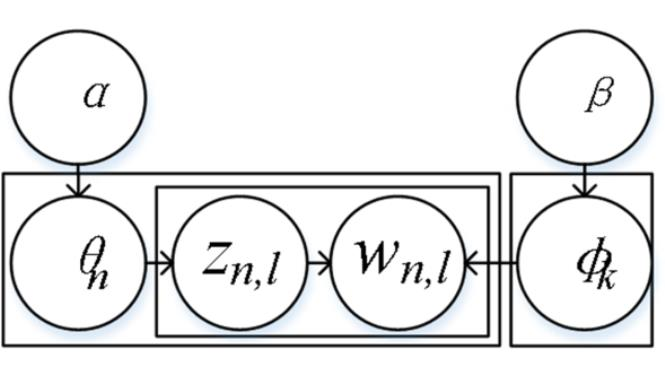
\includegraphics[width=9cm,height=5cm]{res/LDA.jpg}
    \caption{LDA模型图解}
\end{figure} 

如\ref{photo041942}所示,LDA 模型假设每个文档都是多个主题的概率分布,每个主题都是多个分词的概率分布,因此文档-分词概率矩阵可以分解为文档-主题概率矩阵与主题-分词概率矩阵。

笔者也为各位读者提供\ref{table041937}以简明介绍\ref{photo041942}中符号的意义,并提前说明下文将会使用到的一些符号的意义:

\begin{table}[htbp]
    \centering
    \label{table041937}
    \caption{LDA模型符号一览表}
    \begin{tabular}{@{}cc@{}}
    \toprule
    符号            & 意义                        \\ \midrule
    $K$           & 主题总数                      \\
    $k$           & 主题编号                      \\
    $Z_{n,l}$     & 文档$n$中第$l$个分词对应的主题编号      \\
    $\alpha$      & 控制文档-主题分布的超参数/狄利克雷分布先验参数 \\
    $\beta$       & 控制主题-词语分布的超参数/狄利克雷分布先验参数 \\
    $w_{n,l}$     & 是文档$n$中第$l$个分词对应的主题编号     \\
    $\theta _{n}$ & 文档$n$的主题分布                \\
    $\varphi_{k}$ & 主题$k$的词汇分布                \\ \bottomrule
    \end{tabular}
\end{table}

接下来,本文将介绍LDA模型的应用过程,该过程也将参考罗文劼与肖梓良老师编写的《融合知识点与图卷积的在线编程题目推荐算法》\cite{LuoRongHeZhiShiDianYuTuJuanJiDeZaiXianBianChengTiMuTuiJianSuanFa}中对LDA模型应用的过程介绍。

首先,在得到给定题目与分词结果的前提下,可以得到$n$与$w_{n,l}$的值。先验参数$\alpha$与$\beta$则采取经验法则,默认设置为$\frac{1}{K}$ 。当然,还有如网格搜索、贝叶斯优化等其他方式选定更优的先验参数,但本文为研究便利,采用较为简单的方式确定先验参数,不采用其他的方式。读者可以根据自身需要尝试选用其他方式确定先验参数。接下来,则使用吉布斯采样法学习LDA模型中的主题分布$\theta _{n}$,过程如下:

\begin{mgAlgorithm}[吉布采样学习LDA模型过程]
    \item 给定主题总数$K$。
    \item 给每篇文档的每个词汇随机分配主题编号,初始化$Z_{n,l}$。
    \item 利用吉布斯公式对每个词汇进行采样,求出它对应的主题编号,并更新其主题编号$Z_{n,l}$。
    \item 重复上一步骤,直到吉布斯采样收敛或达到迭代次数。
    \item 输出每篇文档的主题分布$\theta _{n}$。
\end{mgAlgorithm}

然后,再取先前分词处理后的题目文本,获得题目集合$N$,再将其与超参数$\alpha$、$\beta$(默认设置为$\frac{1}{K}$)和知识点总数(主题总数)$K$输入LDA模型当中,采用吉布斯采样学习的方式进行参数估计,迭代后输出$N$个题目在$K$个知识点上的概率分布$I_{\varphi}$,如式(\ref{equation041947})所示。

\begin{equation}
    \label{equation041947}
    I_{\varphi}=\left[\begin{array}{cccc}
        i_{11} & i_{12} & \cdots & i_{1 K} \\
        i_{21} & i_{22} & \cdots & i_{2 K} \\
        \cdots & \cdots & \cdots & \cdots \\
        i_{N 1} & i_{N 2} & \cdots & i_{N K}
        \end{array}\right]
\end{equation}

\subsubsection{使用余弦相似度计算相似性结果}

LDA模型将题目视作知识点的集合,每个知识点作为题目的特征。因此,将题目文本映射到知识点的特征向量空间中,即进行了“数学化”。然后,可以通过计算余弦相似度来计算$I_{\varphi}$中每对题目之间的知识相似度,计算过程如下:

设题目$N_{u}$和题目$N_{v}$对应的知识点分布为矩阵$I_{\varphi}$中的两行,则$N_{u}$和$N_{v}$的知识点相似度$ksim(u,v)$可以如式(\ref{equation042004})所示计算:

\begin{equation}
\label{equation042004}
\operatorname{ksim}(u, v)=\frac{\theta_{u} \cdot \theta_{v}}{\left|\theta_{u}\right| \times\left|\theta_{v}\right|}
\end{equation}

其中,$\theta_{u} = \left [ i_{u1},i_{u2}, \dots, i_{uK} \right ] $,$\theta_{v} = \left [ i_{v1},i_{v2}, \dots, i_{vK} \right ] $,且$0 \le ksim(u,v) \le 1$。$ksim(u,v)$越大,则题目$N_{u}$和$N_{v}$的知识点分布越接近,题目相似性越高;反之,则越低。

\subsection{基于模糊数学的难度度量模型}

\begin{figure}[h]
    \centering
    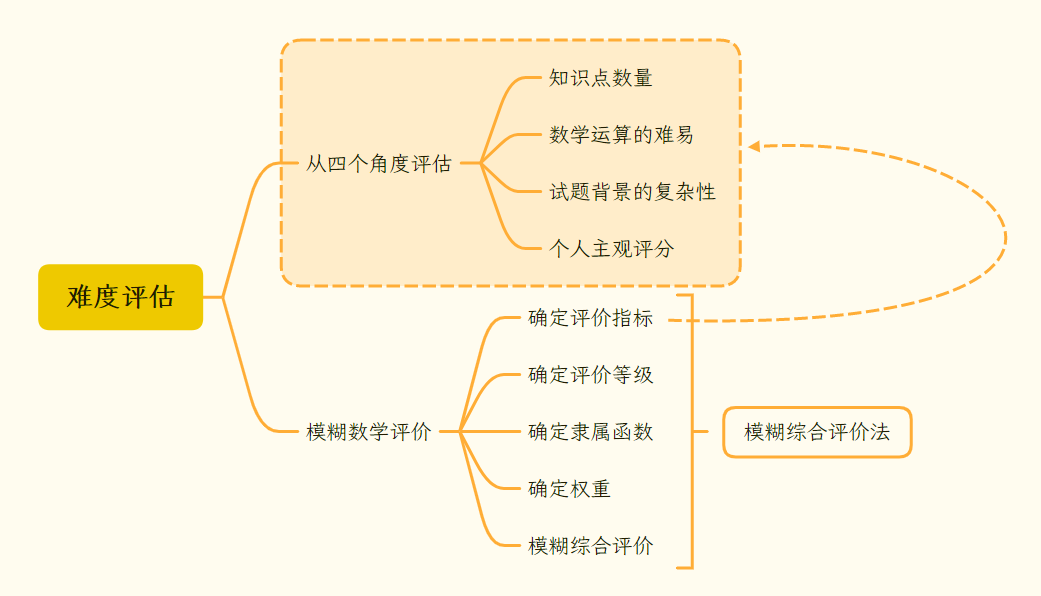
\includegraphics[scale=0.3]{res/figure040041.png}
    \caption{难度度量模型思维导图}
\end{figure}

\subsubsection{确定模糊数学理论方法}

对于一个题目来说,其难度与很多因素有关,并且很难量化地用这些因素来表示一个题目的难度,即一个题目的难度只能用模糊的标准来表示,从而让题目难度度量变得十分困难。

除了根据考试的类型度量题目难度之外,还有根据题目的实际得分率确定题目的难度等其他方法。但是这些方法并不能对度量题目难度提供很好的帮助。如果根据题目的实际得分率确定题目难度,需要采集大量真实的试卷信息。此方法难度大、工作量大,很难保证在有限时间内获得准确的信息。为此需要重新思考其他方法,尽可能很好地对题目难度进行度量。

由此,建立了基于模糊数学的难度度量模型。

相对于研究和处理确定性现象的数学理论和方法,模糊数学是研究和处理模糊性现象的一种数学理论和方法\cite{MoHuShuXue}。为了解决题目难度度量十分困难的问题,提出基于模糊数学的难度度量模型。由于模糊数学的特殊性,其在没有精确标准的题目难度度量方面可以起到很好的度量作用。

综上所述,本文采用模糊数学的理论方法对题目难度进行度量。

\subsubsection{分析题目难度影响因素}

对于一个题目来说,有很多因素能够影响其难度。经分析,主要有四个因素对题目难度产生了影响。

首先,影响一个题目难度最深的因素,是该题目所用到的\textbf{知识点数量}。当一道题要求掌握的知识点数量越多时,学生需要掌握越多的知识点才有可能解决这一问题,即对学生解题的要求越高,从而增加题目的难度。

其次是该题目\textbf{数学运算的难度}。在满足学生发挥稳定、有充足时间、不受外界干扰等理想情况下,该题目数学运算越复杂,学生出错的概率越大,写对该题目的概率就越小,进而让该题目越难。

再其次是\textbf{题目背景的复杂性}。如果题目直接把条件和问题表达清楚,那么这个题目就非常明确;然而很多时候题目中会出现含有故事背景、篇幅较长等各种其他情况,使题目条件不清晰,并且需要学生从中挖掘题目条件和问题。这类题目显然相对于上一种来说,难度更大。

最后是教师的\textbf{个人主观难度判断}。教师对题目更加了解,即对题目难度的确定更加准确。但是考虑到对于不同的教师,其资历和阅题数等各方面不同,从而影响到最终的结果,因而将该因素排在最后。

影响题目难度还有其他因素,如学生知识点实际掌握情况,学生考前的学习情况

\subsubsection{确定难度度量指标}

假定\textbf{题目难度度量因素集}$S_{factor}$,且有:

\begin{equation}
    S_{factor} = \{ s_1, s_2, s_3, s_4 \}
\end{equation}

其中$s_1$、$s_2$、$s_3$和$s_4$为四个影响题目难度的因素,分别代表知识点数量、数学运算的难度、题目背景的复杂性和个人主观难度判断。

\subsubsection{确定难度度量等级}

假定\textbf{难度度量等级}集合$S_{level}$,其中$S_{level}(i)$表示某个因素的得分等级为$i$。

等级越高,某个因素对该题目的难度,相较于其他题目同样的因素与对应的题目的难度来说,贡献越大,即题目越难。

经过考虑,划分为五个等级:
$$S_{level} = \{1, 2, 3, 4, 5\}$$
分别对应得分$1, 2, 3, 4, 5$。

\subsubsection{确定题目难度得分矩阵}

假定\textbf{题目难度得分矩阵}$M_{diff}$,其中$M_{diff}(i, j)$表示第$i$题第$j$个因素的得分等级。

因此,对于所有的$i \geq 1, 1 \leq j \leq 4$,有:

\begin{equation}
M_{diff}(i, j)\in S_{level}
\end{equation}

由于题目难度得分矩阵不确定,并且对于不专业的人来说很难得到准确结果,考虑让多个教师合作完成。

假定有$n$个教师分别完成各自的题目难度得分矩阵,\textbf{所有教师的题目难度矩阵}为一个三维矩阵$M_{diff}'$,其中$M_{diff}'(i, j, k)$表示第$k$个教师认为第$i$题第$j$个因素的得分,且对于所有的$i \geq 1, 1 \leq j \leq 4, 1 \leq k \leq n$,满足:

\begin{equation}
M_{diff}'(i, j, k)\in S_{level}
\end{equation}

得到每个教师的题目难度得分矩阵后,分别对每一题每个因素求教师数量的平均值,设为最终的题目难度得分矩阵,即:

\begin{equation}
    M_{diff}(i, j) = 
    \frac{
        \sum_{k = 1}^{n}M_{diff}'(i, j, k)
    }{n}
\end{equation}

\subsubsection{确定难度度量权重}

假定\textbf{题目难度因素权重序列}$L_{weight}$,其中$L_{weight}(j)$表示第$j$个元素影响题目难度的权重,并且$1 \leq j \leq 4$。

经分析,考虑:

\begin{equation}
    L_{weight} = [4, 3, 2, 1]
\end{equation}

\subsubsection{计算题目难度值}

构建题目难度度量模型之后,可以由此得到\textbf{难度值}$L_{diff}$,其中$L_{diff}(i)$表示第$i$题的难度值,并且满足$i \geq 1$。

由建立的模型可得对应题目难度的加权值为:

\begin{equation}
    L_{diff}(i) = 
    \sum_{j = 1}^{4} \left [ 
        M_{diff}(i, j) \cdot L_{weight}(j)
    \right ]
\end{equation}

\subsubsection{题目难度模糊综合评价}

由于本题目难度度量模型针对的是附件中题库内的所有题目,对于每一题来说,难度值都是相对于题库内所有题目的难度值而言。

假定题目相较于题库中其他题目的难度为\textbf{难度系数}。所有题目的难度系数序列为$L_D$,其中$L_D(i)$表示第$i$题的难度系数,且有$i \geq 1$。

则难度系数的计算方式为:

\begin{equation}
L_D(i) = 
    \frac{
        L_{diff}(i) - \min L_{diff}
    } {
        \max L_{diff} - \min L_{diff}
    }
\end{equation}

其中$\max L_{diff}$为题库中题目最大的难度值、$\min L_{diff}$为题库中题目最小的难度值,并且有$0 \leq L_D(i) \leq 1, i \geq 1$。

至此,题库中所有题目的难度均度量完成,即$L_D$。

\subsection{相似度模型的应用举例——对附件1题库的分类}

\subsubsection{模型应用过程}

为了保证模型的复用性,这里给出评价的步骤。通过对前文中模型的应用,对附件1中的题目进行分类(如图\ref{figure041640})。

\begin{figure}[h]
    \centering
    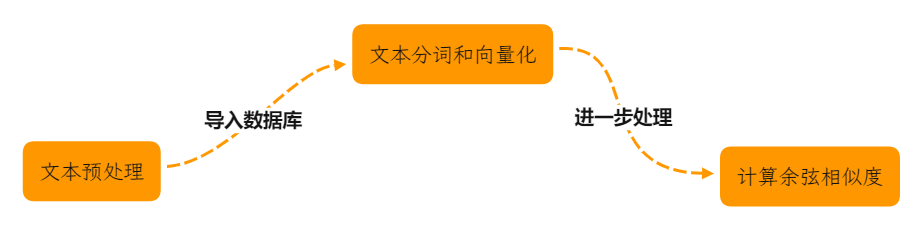
\includegraphics[scale=0.35]{res/figure041640.png}
    \caption{分类步骤}
    \label{figure041640}
\end{figure}

\begin{enumerate}
    \item 文本预处理。格式化已有的数据。让代码1中的程序可以识别题库。处理完成以后,导入到MySQL数据库中;
    \item 文本分词和向量化。将数据导入到数据库中以后,通过LDA模型处理文本,提取特征;
    \item 计算余弦相似度。得到各个题目之间的相似度矩阵。
\end{enumerate}

分类部分结果如表\ref{talbe041618}所示意(完整分类结果见\textbf{附件-题目分类.xlsx})。

\begin{table}[h]
    \label{talbe041618}
    \caption{分类结果}
    \centering
    \begin{tabular}{@{}cccccc@{}}
        \toprule
        \quad \quad 一 \quad \quad   & \quad \quad 二 \quad \quad  & \quad \quad 三 \quad \quad   & \quad \quad 四 \quad \quad                  & \quad \quad 五 \quad \quad    & \quad \quad …… \quad \quad                  \\ \midrule
        P001 & P002 & P007 & P015                 & P023 &                      \\
        P005 & P003 & P010 & P071                 & P024 &                      \\
        P008 & P004 & P014 & P089                 & P028 &                      \\
        P009 & P006 & P026 & P097                 & P032 &                      \\
        P016 & P011 & P034 &  -                   & P043 &                      \\
        P019 & P012 & P040 &  -                   & P050 &                      \\
        P021 & P013 & P044 &  -                   & P054 &                      \\
        P025 & P018 & P047 &  -                   & P068 &                      \\
        P027 & P020 & P052 &  -                   & P075 &                      \\
        P029 & P022 & P053 &  -                   & P081 &                      \\
        P033 & P030 & P055 &  -                   & P084 &                      \\
        P036 & P035 & P065 &  -                   & P087 &                      \\
        P038 & P037 & P080 &  -                   & P088 &                      \\
        P039 & P046 & P083 &  -                   & -    &                      \\
        P041 & P049 & P085 &  -                   & -    &                      \\
        P048 & P051 & P091 & \multicolumn{1}{l}{} &     & \multicolumn{1}{l}{} \\
        \multicolumn{6}{c}{……}                                                  \\ \bottomrule
        \end{tabular}
\end{table}

实际上,对于该种分类方法而言,越大的题库就有着越好的分类效果。更大的题库意味着更大的材料库,如此巨大的材料库对模型的意义就是能够拟合出更加合理、更加符合现实的结论。


\subsubsection{对于大规模题库}

该方法的复杂度主要集中在文本预处理和文本分词向量化这两个步骤中。对于前者,在做出优化判断之前,需要优质的数据集,如果数据集不够优质,那么前期就要花费大量的时间整合原文本,所以优质的数据集可以节省大量的时间。

综上所述,\textbf{影响该算法复杂的因素主要是原文的质量和数据处理时的技巧相关,在一定程度上,可以用于大题库中。}

\subsection{难度评估模型的应用举例——对附件2的难度分析}

\subsubsection{分析题目难度}

利用本模型,对题库里的所有题目进行了一次难度模糊综合评价。附件中名为“题目难度得分矩阵.xlsx”的三个文件,为团队三个成员对所有题目相应的难度评价结果。而在名为“题目难度系数计算.xlsx”的文件内:“题目难度因素权重序列”这一工作表为模型四个影响题目难度的因素对应的权重;“题目难度系数计算”这一工作表为,对三个题目难度得分矩阵求得最终的题目难度得分矩阵,并计算出每一题对应的难度值和难度系数;“最终结果”这一工作表为整合上述计算后最终的题目对应的难度系数。表\ref{tableDiff}为附件二中题目编号及其对应的难度系数。

\begin{table}[htbp]
    \centering
    \label{tableDiff}
    \caption{附件二题目对应难度系数}
    \begin{tabular}{@{}cc@{}}
    \toprule
    \quad\quad\quad\quad\quad题目编号\quad\quad\quad\quad\quad & \quad\quad\quad\quad\quad难度系数\quad\quad\quad\quad\quad\\ \midrule
    Q001 & 0.3860 \\
    Q002 & 0.7193 \\
    Q003 & 0.5088 \\
    Q004 & 0.6842 \\
    Q005 & 0.4386 \\
    Q006 & 0.2105 \\
    Q007 & 0.4912 \\
    Q008 & 0.3509 \\
    Q009 & 0.3333 \\
    Q010 & 0.5439 \\ \bottomrule
    \end{tabular}
\end{table}

其他数据见“附件-题目难度系数计算.zip”文件中的“最终结果”。

\subsubsection{寻找题目难度相似的题目}

对“题目难度系数计算.xlsx”文件中的“最终结果”中,以“难度系数”为关键字降序排序。容易看出,以难度为标准时,附件二的题目与附件一中的相似题目的对应关系如表\ref{tablesmr}。

\begin{table}[htbp]
    \centering
    \label{tablesmr}
    \caption{以难度为标准的相似题目}
    \begin{tabular}{@{}cc@{}}
    \toprule
    \quad\quad\quad\quad\quad题目编号\quad\quad\quad\quad\quad & \quad\quad\quad\quad\quad相似题目\quad\quad\quad\quad\quad\\ \midrule
    Q001 & P020, P043, P077, P092 \\
    Q002 & P063 \\
    Q003 & P031, P053, P016, P030 \\
    Q004 & P089, P059 \\
    Q005 & P067 \\
    Q006 & P097, P078 \\
    Q007 & P030, P012, P015, P023 \\
    Q008 & P094, P019, P035, P061 \\
    Q009 & P013, P038 \\
    Q010 & P011, P048 \\ \bottomrule
    \end{tabular}
\end{table}

其他数据见“题目难度系数计算.xlsx”文件中的“最终结果”。

\subsubsection{计算算法复杂度}

假定有$n$名教师共同评估一个题库里的$m$道题目,在所有教师完成各自的题目难度矩阵后,计算最终的题目难度得分矩阵的时间复杂度为$O(mn)$。

由于有$m$道题目,并且影响题目难度因素个数为常数,因此计算完所有题目的难度值的时间复杂度为$O(m)$。

计算$m$道题目的难度系数时,获取最大最小难度值的时间复杂度为$O(m)$,最后计算难度系数的时间复杂度为$O(m)$。因此最终计算所有题目的难度系数的时间复杂度为$O(m + m)$,即等价于$O(m)$。

综上所述,本基于模糊数学的难度度量模型的总时间复杂度为$O(mn)$(其中$m$表示题库中题目的数量,$n$表示评估题目的教师总人数)。

由于$m$的值越大,参与评估的教师人数越多,得到的结果越精确。即对于更大规模的题库时,如果对精度要求不高,则可以视为适用于更大规模的题库;但是对结果精度要求高的话,本模型将会花费较长的时间求得结果。

总之,\textbf{如果对结果精度要求不高,则可以适用于更大规模的题库;否则将难以适应并需要花费较长时间获取结果。}

% ============================================================
%
% 模型的评价与改进
%
% ============================================================

\section{模型的评价与改进}

\subsection{模型的优点}

\subsubsection{基于LDA的相似性度量模型}

\begin{itemize}
    \item 题库的规模越大,题目的相似性判断越准确;
    \item 充分考虑了文本和问题之间的关联,提高了题目之间相似性度量的准确性;
    \item 能够处理高维稀疏数据:在文本相似性计算中,经常出现高维稀疏的数据表示,这对传统的文本相似度模型构成了挑战。
\end{itemize}

\subsubsection{基于模糊数学的难度度量模型}

\begin{itemize}
    \item 避免了题目难度非黑即白的二元评价,通过模糊综合评价方法给予题目难度更多的可能性;
    \item 通过模糊数学的判断,很好的体现了人类的思维过程;
    \item 提高了决策质量
\end{itemize}

\subsection{模型的缺点}

\subsubsection{基于LDA的相似性度量模型}

\begin{itemize}
    \item LDA模型是一种基于词袋模型的统计模型,它忽略了词汇之间的顺序和语法结构,而这些信息在数学应用题中可能非常重要;
    \item LDA模型假设每个文档由多个主题组成,每个主题又由多个词汇组成。这种假设在大多数自然语言文本中是合理的,但在度量小学数学应用题的相似性时可能会产生问题。因为数学应用题通常只涉及一个或几个主题,而这些主题可能只包含少量的词汇,这使得LDA模型很难从中提取有用的信息;
    \item LDA模型需要大量的数据来进行训练,否则容易出现过拟合的问题。在小样本数据情况下,LDA模型可能会将噪声误认为是有意义的主题,从而导致相似性度量不准确。
\end{itemize}

\subsubsection{基于模糊数学的难度度量模型}

\begin{itemize}
    \item 该模型还不能完全撇清人的主观性,只是对人的主观性做出了一定的限制;
    \item 该模型的应用需要大量的人力一个个给题库中的题目评价才可以正常使用,在更大的题库中成本很高;
    \item 该模型的评价体系完全基于专家过往的经验,没有坐落在可信的理论之上。
\end{itemize}

\subsection{模型的改进}

\subsubsection{基于LDA的相似性度量模型}

\begin{itemize}
    \item 使用更加复杂的语义模型:例如基于神经网络的自然语言处理模型,这些模型可以充分利用词汇之间的语义和上下文信息,提高相似性度量的准确性;
    \item 优化主题的数量和词汇的权重:LDA模型中,主题的数量和词汇的权重对相似性度量的结果有很大影响。因此,可以通过对主题数量进行调整,或者对词汇的权重进行加权,来减少误差;
    \item 增加样本数据量:在小样本数据情况下,LDA模型容易出现过拟合的问题,从而导致相似性度量不准确。因此,可以通过增加样本数据量来解决这个问题,例如通过扩充数据集或者使用数据增强等方法。
\end{itemize}

\subsubsection{基于模糊数学的难度度量模型}

\begin{itemize}
    \item 用AI评价代替人工评价。这样做有两个好处,首先AI评价相比于人工评价更加客观,其次AI评价相比于人工评价成本更低,效率更高;
    \item 寻找一种更为合理的小学知识体系,以这个体系为基础,再进行题目难度度量。
\end{itemize}